
%%%%%%%%%%%%%%%%%%%%%%%%%%%%%%%%%%%%%%%%%
% Short Sectioned Assignment LaTeX Template Version 1.0 (5/5/12)
% This template has been downloaded from: http://www.LaTeXTemplates.com
% Original author:  Frits Wenneker (http://www.howtotex.com)
% License: CC BY-NC-SA 3.0 (http://creativecommons.org/licenses/by-nc-sa/3.0/)
%%%%%%%%%%%%%%%%%%%%%%%%%%%%%%%%%%%%%%%%%

%----------------------------------------------------------------------------------------
%	PACKAGES AND OTHER DOCUMENT CONFIGURATIONS
%----------------------------------------------------------------------------------------

\documentclass[paper=a4, fontsize=11pt]{scrartcl} % A4 paper and 11pt font size

% ---- Entrada y salida de texto -----

\usepackage[T1]{fontenc} % Use 8-bit encoding that has 256 glyphs
\usepackage[utf8]{inputenc}
%\usepackage{fourier} % Use the Adobe Utopia font for the document - comment this line to return to the LaTeX default

% ---- Idioma --------

\usepackage[spanish, es-tabla]{babel} % Selecciona el español para palabras introducidas automáticamente, p.ej. "septiembre" en la fecha y especifica que se use la palabra Tabla en vez de Cuadro

% ---- Otros paquetes ----

\usepackage{url} % ,href} %para incluir URLs e hipervínculos dentro del texto (aunque hay que instalar href)
\usepackage{amsmath,amsfonts,amsthm} % Math packages
%\usepackage{graphics,graphicx, floatrow} %para incluir imágenes y notas en las imágenes
\usepackage{graphics,graphicx, float} %para incluir imágenes y colocarlas
\usepackage{movie15}

% Para hacer tablas comlejas
%\usepackage{multirow}
%\usepackage{threeparttable}

%\usepackage{sectsty} % Allows customizing section commands
%\allsectionsfont{\centering \normalfont\scshape} % Make all sections centered, the default font and small caps

\usepackage{fancyhdr} % Custom headers and footers

\pagestyle{fancyplain} % Makes all pages in the document conform to the custom headers and footers
\fancyhead{} % No page header - if you want one, create it in the same way as the footers below
\fancyfoot[L]{} % Empty left footer
\fancyfoot[C]{} % Empty center footer
\fancyfoot[R]{\thepage} % Page numbering for right footer
\renewcommand{\headrulewidth}{0pt} % Remove header underlines
\renewcommand{\footrulewidth}{0pt} % Remove footer underlines
\setlength{\headheight}{13.6pt} % Customize the height of the header

\numberwithin{equation}{section} % Number equations within sections (i.e. 1.1, 1.2, 2.1, 2.2 instead of 1, 2, 3, 4)
\numberwithin{figure}{section} % Number figures within sections (i.e. 1.1, 1.2, 2.1, 2.2 instead of 1, 2, 3, 4)
\numberwithin{table}{section} % Number tables within sections (i.e. 1.1, 1.2, 2.1, 2.2 instead of 1, 2, 3, 4)

\setlength\parindent{0pt} % Removes all indentation from paragraphs - comment this line for an assignment with lots of text

\newcommand{\horrule}[1]{\rule{\linewidth}{#1}} % Create horizontal rule command with 1 argument of height
\usepackage[breaklinks=true]{hyperref}
\usepackage{bookmark}
\usepackage{wasysym}
\usepackage{subcaption}
\usepackage[dvipsnames]{xcolor}
\usepackage{amssymb}
\usepackage{color}
\usepackage{listings}
\usepackage{upgreek} % para poner letras griegas sin cursiva
\usepackage{cancel} % para tachar
\usepackage{mathdots} % para el comando \iddots
\usepackage{mathrsfs} % para formato de letra
\usepackage{stackrel} % para el comando \stackbin
\lstdefinestyle{cmas}
{ %
	language=C++,                % elegir el lenguaje del código
	stringstyle=\color{blue}\ttfamily,,
	basicstyle=\normalsize\ttfamily,       % el tamaño del font a usar para el código
	numbers=left,                   % dónde poner los números de línea 
	numberstyle=\footnotesize,      % tamaño de font usados para los números de línea 
	stepnumber=1,                   % el paso de numeración
	numbersep=8pt,                  % distancia del numero de línea y la línea
	backgroundcolor=\color{white},  % color de fondo, para usarlo hay que agregar  \usepackage{color}
	showspaces=false,               % mostrar espacios en blanco ?
	showstringspaces=false,         % subrayar espacios con cadenas?   
	 showtabs=false,                 % mostrar taba usando cadenas? 
	frame=single,           			% enmarcar el código?  
	tabsize=2,          				% sets default tabsize to 2 spaces?
	keywordstyle=\color{MidnightBlue}\ttfamily\bfseries,
	commentstyle=\color{OliveGreen}\ttfamily,
	morecomment=[l][\color{OliveGreen}]{\#},
	captionpos=b,           % sets the caption-position to bottom?
	breaklines=true,        % sets automatic line breaking?
	breakatwhitespace=false,    % sets if automatic breaks should only happen at whitespace ?
	title=\lstname,
	escapeinside={\%*}{*)}          % if you want to add a comment within your code
}

\lstdefinestyle{payt}
{ %
	language=Python,                % elegir el lenguaje del código
	stringstyle=\color{blue}\ttfamily,,
	basicstyle=\normalsize\ttfamily,       % el tamaño del font a usar para el código
	numbers=left,                   % dónde poner los números de línea 
	numberstyle=\footnotesize,      % tamaño de font usados para los números de línea 
	stepnumber=1,                   % el paso de numeración
	numbersep=8pt,                  % distancia del numero de línea y la línea
	backgroundcolor=\color{white},  % color de fondo, para usarlo hay que agregar  \usepackage{color}
	showspaces=false,               % mostrar espacios en blanco ?
	showstringspaces=false,         % subrayar espacios con cadenas?   
	showtabs=false,                 % mostrar taba usando cadenas? 
	frame=single,           			% enmarcar el código?  
	tabsize=2,          				% sets default tabsize to 2 spaces?
	keywordstyle=\color{MidnightBlue}\ttfamily\bfseries,
	commentstyle=\color{OliveGreen}\ttfamily,
	morecomment=[l][\color{OliveGreen}]{\#},
	captionpos=b,           % sets the caption-position to bottom?
	breaklines=true,        % sets automatic line breaking?
	breakatwhitespace=false,    % sets if automatic breaks should only happen at whitespace ?
	title=\lstname,
	escapeinside={\%*}{*)}          % if you want to add a comment within your code
}

\definecolor{light-gray}{gray}{0.85}

\lstdefinestyle{fich}
{ %
	language=Bash,                % elegir el lenguaje del código
	stringstyle=\color{black}\texttt,
	basicstyle=\normalsize\ttfamily,       % el tamaño del font a usar para el código	
	numbers=left,                   % dónde poner los números de línea 
	numberstyle=\footnotesize,      % tamaño de font usados para los números de línea 
	stepnumber=1,                   % el paso de numeración
	numbersep=8pt,                  % distancia del numero de línea y la línea
	backgroundcolor=\color{light-gray},  % color de fondo, para usarlo hay que agregar  \usepackage{color}
	showspaces=false,               % mostrar espacios en blanco ?
	showstringspaces=false,         % subrayar espacios con cadenas?   
	showtabs=false,                 % mostrar taba usando cadenas? 
%	frame=single,           			% enmarcar el código?  
	tabsize=2,          				% sets default tabsize to 2 spaces?
	captionpos=b,           % sets the caption-position to bottom?
	breaklines=true,        % sets automatic line breaking?
	breakatwhitespace=false,    % sets if automatic breaks should only happen at whitespace ?
	title=\lstname,
	escapeinside={\%*}{*)}          % if you want to add a comment within your code
}

\lstset{literate=
  {á}{{\'a}}1 {é}{{\'e}}1 {í}{{\'i}}1 {ó}{{\'o}}1 {ú}{{\'u}}1
  {Á}{{\'A}}1 {É}{{\'E}}1 {Í}{{\'I}}1 {Ó}{{\'O}}1 {Ú}{{\'U}}1
  {à}{{\`a}}1 {è}{{\`e}}1 {ì}{{\`i}}1 {ò}{{\`o}}1 {ù}{{\`u}}1
  {À}{{\`A}}1 {È}{{\'E}}1 {Ì}{{\`I}}1 {Ò}{{\`O}}1 {Ù}{{\`U}}1
  {ä}{{\"a}}1 {ë}{{\"e}}1 {ï}{{\"i}}1 {ö}{{\"o}}1 {ü}{{\"u}}1
  {Ä}{{\"A}}1 {Ë}{{\"E}}1 {Ï}{{\"I}}1 {Ö}{{\"O}}1 {Ü}{{\"U}}1
  {â}{{\^a}}1 {ê}{{\^e}}1 {î}{{\^i}}1 {ô}{{\^o}}1 {û}{{\^u}}1
  {Â}{{\^A}}1 {Ê}{{\^E}}1 {Î}{{\^I}}1 {Ô}{{\^O}}1 {Û}{{\^U}}1
  {œ}{{\oe}}1 {Œ}{{\OE}}1 {æ}{{\ae}}1 {Æ}{{\AE}}1 {ß}{{\ss}}1
  {ű}{{\H{u}}}1 {Ű}{{\H{U}}}1 {ő}{{\H{o}}}1 {Ő}{{\H{O}}}1
  {ç}{{\c c}}1 {Ç}{{\c C}}1 {ø}{{\o}}1 {å}{{\r a}}1 {Å}{{\r A}}1
  {€}{{\EUR}}1 {£}{{\pounds}}1
  {ñ}{{\~n}}1
}

\hypersetup{
    colorlinks=true,
    linkcolor=black,
    filecolor=magenta,      
    urlcolor=blue,
    pdftitle={ISE: Práctica 3 - Mario Rodríguez Ruiz},
    bookmarks=true,
    citecolor=blue,
}



%----------------------------------------------------------------------------------------
%	TÍTULO Y DATOS DEL ALUMNO
%----------------------------------------------------------------------------------------

\title{	
\normalfont \normalsize 
\textsc{\textbf{Ingeniería de Servidores (2016-2017)} \\ Subgrupo A1 \\ Grado en Ingeniería Informática\\ Universidad de Granada} \\ [25pt] % Your university, school and/or department name(s)
\horrule{0.5pt} \\[0.4cm] % Thin top horizontal rule
\huge Práctica 4: Benchmarks \\ % The assignment title
\horrule{2pt} \\[0.5cm] % Thick bottom horizontal rule
}

\author{Mario Rodríguez Ruiz} % Nombre y apellidos

\date{\normalsize\today} % Incluye la fecha actual

%----------------------------------------------------------------------------------------
% DOCUMENTO
%----------------------------------------------------------------------------------------

\begin{document}

\maketitle % Muestra el Título

\newpage %inserta un salto de página

\tableofcontents % para generar el índice de contenidos

\listoffigures

\listoftables

\newpage

%----------------------------------------------------------------------------------------
%	Cuestión 1
%----------------------------------------------------------------------------------------

\section{Cuestión 1: PHORONIX SUITE}
\subsection{Seleccione, instale y ejecute uno, comente los resultados.
	Atención: no es lo mismo un benchmark que una suite, instale un
	benchmark}

\subsubsection{Descarga e instalación de PHORONIX SUITE}

Se ha instalado en CentOS 7 la última versión de la suite (descargada desde su página oficial \cite{enlace2}), pero esta guía serviría para cualquier otra cambiando el número de versión de ésta en los comandos.
\\
\vspace{-3.8pt}
En primer lugar se descargan e instalan las dependencias necesarias de este paquete \cite{enlace1}, para poder visualizar los resultados desde el navegador, con la siguiente orden y como muestra la Figura \ref{fig:figura1-1}:
\begin{lstlisting}[style=fich]
$ yum install wget php-cli bzip2 php-xml -y
\end{lstlisting}
\vspace{-28pt}
\begin{figure}[H] %con el [H] le obligamos a situar aquí la figura
	\centering
	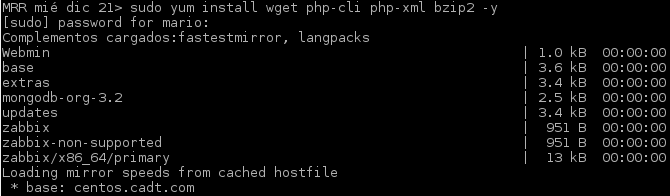
\includegraphics[scale=0.8]{figuras/ejercicio1/figura1-1.png} 
	\caption{Instalación de depencencias de Phoronix Suite} 
	\label{fig:figura1-1}
\end{figure}
\vspace{-11pt}
A continuación se descarga la versión deseada de la suite, en este caso la \textbf{6.8.0} que en este momento es la más reciente.

Para ello se utiliza el comando siguiente y que puede verse en la Figura \ref{fig:figura1-2}:

\begin{lstlisting}[style=fich]
$ wget http://www.phoronix-test-suite.com/download.php?file=phoronix-test-suite-6.8.0 -O phoronix-test-suite_6.8.0.tar.gz
\end{lstlisting}
\vspace{-28pt}
\begin{figure}[H] %con el [H] le obligamos a situar aquí la figura
	\centering
	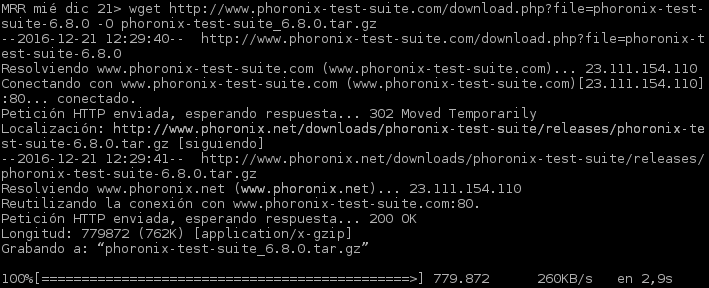
\includegraphics[scale=0.7]{figuras/ejercicio1/figura1-2.png} 
	\caption{Descarga de Phoronix Suite} 
	\label{fig:figura1-2}
\end{figure}

Con la suite descargada, ya solo falta proceder con la instalación. Para ello se descomprime el fichero que se ha descargado, se ubica la consola en la nueva carpeta creada y se ejecuta el script de instalación.

\begin{figure}[H] %con el [H] le obligamos a situar aquí la figura
	\centering
	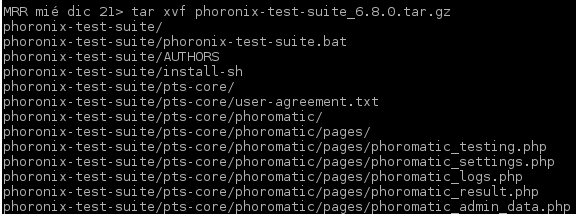
\includegraphics[scale=1]{figuras/ejercicio1/figura1-3.png} 
	\caption{Descomprensión del fichero descargado Phoronix Suite} 
	\label{fig:figura1-3}
\end{figure}

Los pasos son los que se muestran a continuación y que también se presentan en las Figuras \ref{fig:figura1-3} y \ref{fig:figura1-4} \cite{enlace1}:
\begin{lstlisting}[style=fich]
$ tar xvf phoronix-test-suite_6.2.2.tar.gz
$ cd phoronix-test-suite/
$ ./install-sh
\end{lstlisting}
\vspace{-28pt}
\begin{figure}[H] %con el [H] le obligamos a situar aquí la figura
	\centering
	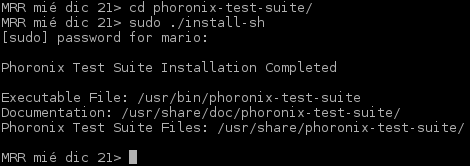
\includegraphics[scale=1]{figuras/ejercicio1/figura1-4.png} 
	\caption{Descomprensión del fichero descargado Phoronix Suite} 
	\label{fig:figura1-4}
\end{figure}

%En la Figura \ref{fig:figura1} se muestra el contenido actual de este fichero en la máquina CentOS.
%\begin{figure}[H] %con el [H] le obligamos a situar aquí la figura
%	\centering
%	\includegraphics[scale=0.9]{figuras/figura1.png} 
%	\caption{Contenido del fichero \textbf{/var/log/yum.log} en CentOS} 
%	\label{fig:figura1}
%\end{figure}

\subsubsection{Listado de benchmark e instalación de uno concreto}

Una vez la suite instalada, se puede comprobar los benchmark de los que dispone el sistema. Para ello se utiliza la siguiente orden (puede verse el resultado parcial del listado en las Figuras \ref{fig:figura1-5} y \ref{fig:figura1-6}):
\begin{lstlisting}[style=fich]
$ /usr/bin/phoronix-test-suite list-available-suites
\end{lstlisting}
\vspace{-28pt}

\begin{figure}[H] %con el [H] le obligamos a situar aquí la figura
	\centering
	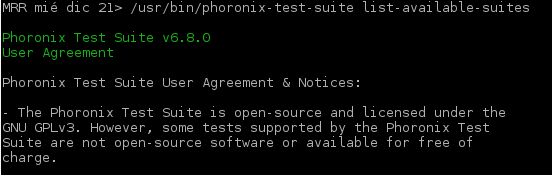
\includegraphics[scale=1]{figuras/ejercicio1/figura1-5.png} 
	\caption{Listado de benchmarks de Phoronix Suite} 
	\label{fig:figura1-5}
\end{figure}

En este estudio se ha visto interesante la opción de hacerle la prueba del test a la memoria del sistema. Antes de poder realizar la ejecución hay que instalar el benchmark necesario para este caso (\textbf{pts/memory}).

\begin{figure}[H] %con el [H] le obligamos a situar aquí la figura
	\centering
	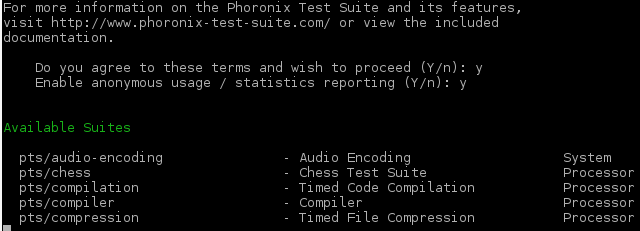
\includegraphics[scale=0.9]{figuras/ejercicio1/figura1-6.png} 
	\caption{Listado de benchmarks de Phoronix Suite} 
	\label{fig:figura1-6}
\end{figure}

Para esto se ejecuta la siguiente orden:
\begin{lstlisting}[style=fich]
$ phoronix-test-suite install pts/memory
\end{lstlisting}
\vspace{-20pt}
El resultado de esta instalación se muestra en la Figura \ref{fig:figura1-10}.
\begin{figure}[H] %con el [H] le obligamos a situar aquí la figura
	\centering
	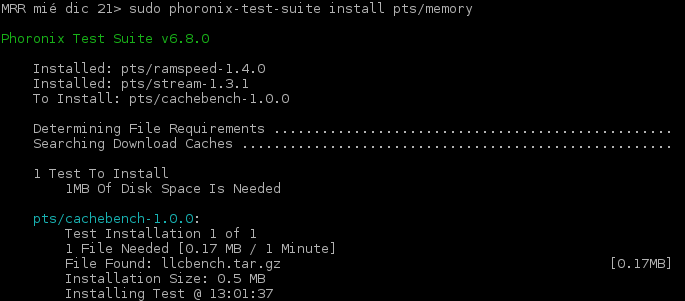
\includegraphics[scale=0.8]{figuras/ejercicio1/figura1-10.png} 
	\caption{Instalación de un benchmark de memoria} 
	\label{fig:figura1-10}
\end{figure}

\subsubsection{Ejecución del benchmark}

Ahora que ya se encuentra instalado en el sistema el benchmark que se va a ejecutar, solo hay que lanzarlo.

Esto se consigue a través de la siguiente orden:
\begin{lstlisting}[style=fich]
$ phoronix-test-suite benchmark pts/memory
\end{lstlisting}
\vspace{-28pt}
\begin{figure}[H] %con el [H] le obligamos a situar aquí la figura
	\centering
	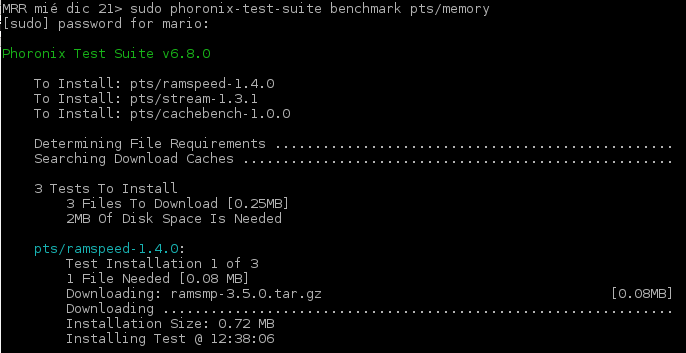
\includegraphics[scale=0.8]{figuras/ejercicio1/figura1-7.png} 
	\caption{Ejecución de un benchmark de memoria} 
	\label{fig:figura1-7}
\end{figure}

Las Figuras \ref{fig:figura1-10} y \ref{fig:figura1-11} muestran el proceso de ejecución del benchmark en cuestión. Además en la Figura \ref{fig:figura1-11} se ve los parámetros que hay que especificar antes de que comience la ejecución del mismo. Éstos son: el de aprobación a que se guarden los resultados, el nombre del fichero que se generará y una pequeña descripción de éste.

\begin{figure}[H] %con el [H] le obligamos a situar aquí la figura
	\centering
	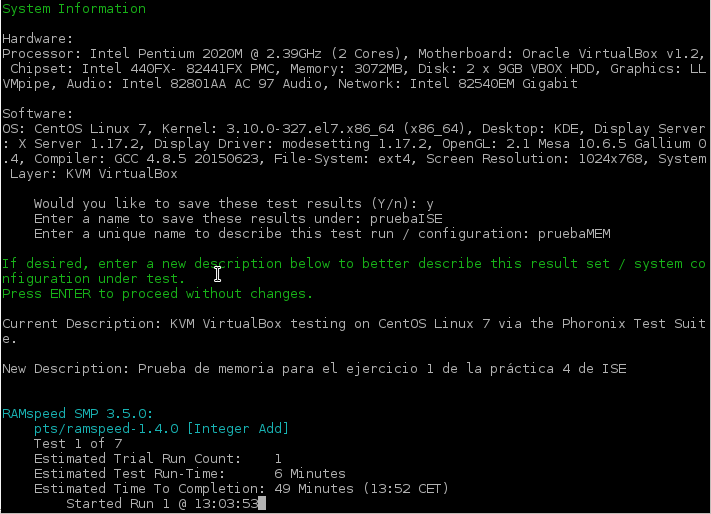
\includegraphics[scale=0.8]{figuras/ejercicio1/figura1-11.png} 
	\caption{Ejecución de un benchmark de memoria} 
	\label{fig:figura1-11}
\end{figure}

En este caso la ejecución de la prueba durará en torno a los 49 minutos. Esta información junto a un pequeño resumen de las características del sistema en el que se realizará ésta también es mostrada en la Figura \ref{fig:figura1-11}.\\

Una vez finalizado el benchmark, se preguntará si se desean visualizar los resultados desde el navegador (es por ello que requería la dependencia de \textbf{php} en la instalación de la suite) como se ve en la Figura \ref{fig:figura1-12}. 
\\

En este caso se ha aceptado y se han mostrado desglosados tal y como aparecen en la Figura \ref{fig:figura1-13}, en la que se muestra una página principal con las características del sistema y un resumen de éstos.

\begin{figure}[H] %con el [H] le obligamos a situar aquí la figura
	\centering
	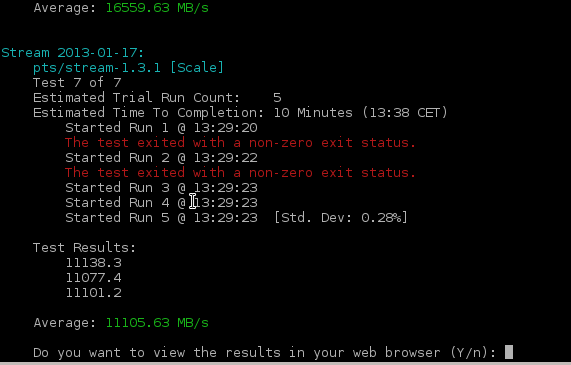
\includegraphics[scale=0.9]{figuras/ejercicio1/figura1-12.png} 
	\caption{Finalizada la ejecución del benchmark de memoria} 
	\label{fig:figura1-12}
\end{figure}

\begin{figure}[H] %con el [H] le obligamos a situar aquí la figura
	\centering
	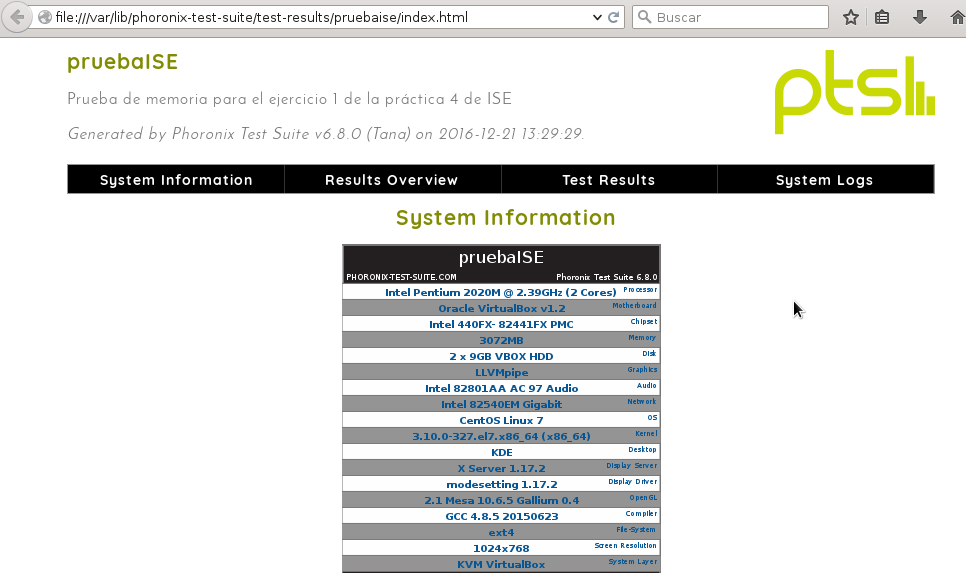
\includegraphics[scale=0.6]{figuras/ejercicio1/figura1-13.png} 
	\caption{Resultados del benchmark de memoria} 
	\label{fig:figura1-13}
\end{figure}


\subsubsection{Resultados}

Las cuatro primeras pruebas que se han realizado sobre el sistema han sido las proporcionadas por \textbf{RAMspeed} \cite{enlace3}, una herramienta utilizada para medir el rendimiento de memoria. La versión \textbf{SMP} es compatible solamente con para máquinas multiprocesador que ejecutan sistemas operativos tipo UNIX.
\\

Ésta utilidad, en primer lugar ha ejecutado una prueba basada en \textbf{integer add} (Figura \ref{fig:figura1-1-1}) .

\begin{figure}[H] %con el [H] le obligamos a situar aquí la figura
	\centering
	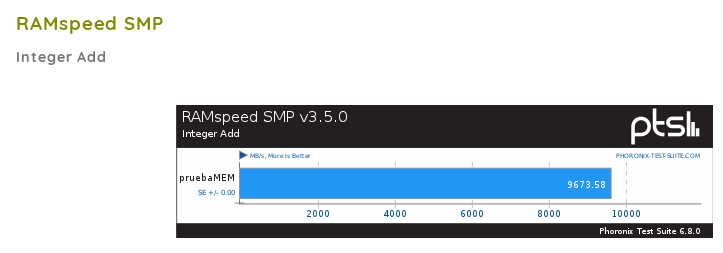
\includegraphics[scale=0.8]{figuras/ejercicio1/resultados/figura1-1-1.png} 
	\caption{Integer add - RAMspeed} 
	\label{fig:figura1-1-1}
\end{figure}

En segundo lugar, ha realizado prueba basada en \textbf{integer copy} (Figura \ref{fig:figura1-1-2})

\begin{figure}[H] %con el [H] le obligamos a situar aquí la figura
	\centering
	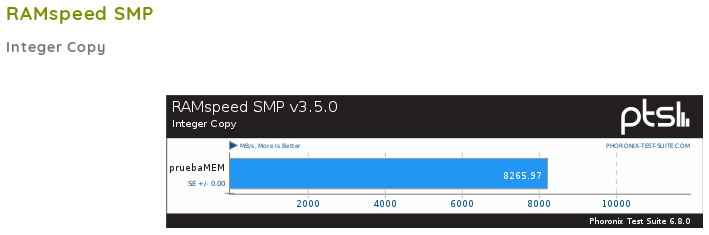
\includegraphics[scale=0.8]{figuras/ejercicio1/resultados/figura1-1-2.png} 
	\caption{Integer copy - RAMspeed} 
	\label{fig:figura1-1-2}
\end{figure}

En tercer lugar, ha realizado prueba basada en \textbf{integer scale} (Figura \ref{fig:figura1-1-3})

\begin{figure}[H] %con el [H] le obligamos a situar aquí la figura
	\centering
	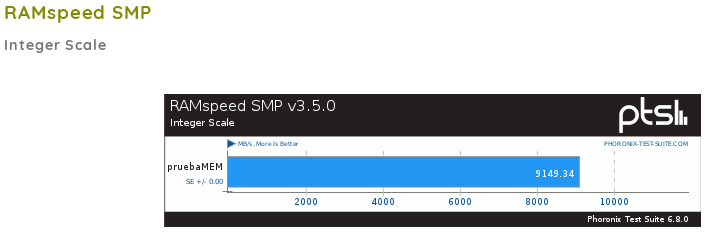
\includegraphics[scale=0.8]{figuras/ejercicio1/resultados/figura1-1-3.png} 
	\caption{Integer scale - RAMspeed} 
	\label{fig:figura1-1-3}
\end{figure}

En cuarto y último lugar, ha realizado prueba basada en \textbf{Floating-Point add} (Figura \ref{fig:figura1-1-4})

\begin{figure}[H] %con el [H] le obligamos a situar aquí la figura
	\centering
	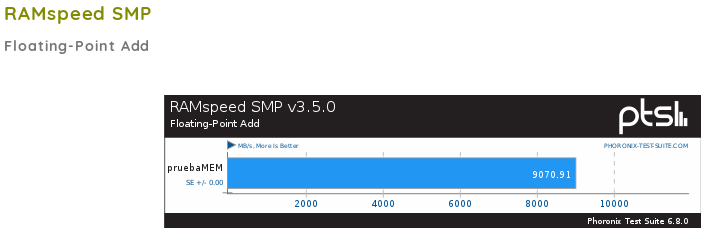
\includegraphics[scale=0.8]{figuras/ejercicio1/resultados/figura1-1-4.png} 
	\caption{Floating-Point add - RAMspeed} 
	\label{fig:figura1-1-4}
\end{figure}


Estas cuatro pruebas son simulaciones sintéticas, no obstante se relacionan con gran cantidad de aplicaciones reales en la actualidad \cite{enlace3}. 
\\

Buscando en las páginas de referencia del autor del benchmark y relacionadas se ha encontrado escasa documentación sobre ésta. El autor en su página da por sentado los conocimientos de quienes aplican dicho test por lo que no detalla apenas su funcionamiento, nombrando las pruebas que hace y poco más.\\

Ojeando su código fuente lo que se ha podido ver es que utiliza bloques completos de memoria para hacer operaciones con ellos y más tarde calcula el tiempo de desarrollo de las mismas.
\\

Aparecen muchas complicaciones en este estudio cuando ni en el propio fichero fuente no aparece la más mínima documentación, es por ello que tan solo queda estudiar el contenido de éste e intentar comprenderlo todo. Parte del \textbf{Floating-point add} se adjunta a continuación.

\begin{lstlisting}[style=cmas]
a = (F64 *) malloc(blk);
b = (F64 *) malloc(blk);
	
for(i = 0; i < blk/sizeof(F64); i++) a[i] = PI;

gettimeofday(&time, NULL);
start  = time.tv_sec;
ustart = time.tv_usec;

while(passnum--) {
	for(i = 0; i < blk/sizeof(F64); i += 32) {
		b[i] = a[i];        b[i+1] = a[i+1];
		b[i+2] = a[i+2];    b[i+3] = a[i+3];
		b[i+4] = a[i+4];    b[i+5] = a[i+5];
		b[i+6] = a[i+6];    b[i+7] = a[i+7];
		b[i+8] = a[i+8];    b[i+9] = a[i+9];
		b[i+10] = a[i+10];  b[i+11] = a[i+11];
		b[i+12] = a[i+12];  b[i+13] = a[i+13];
		b[i+14] = a[i+14];  b[i+15] = a[i+15];
		b[i+16] = a[i+16];  b[i+17] = a[i+17];
		b[i+18] = a[i+18];  b[i+19] = a[i+19];
		b[i+20] = a[i+20];  b[i+21] = a[i+21];
		b[i+22] = a[i+22];  b[i+23] = a[i+23];
		b[i+24] = a[i+24];  b[i+25] = a[i+25];
		b[i+26] = a[i+26];  b[i+27] = a[i+27];
		b[i+28] = a[i+28];  b[i+29] = a[i+29];
		b[i+30] = a[i+30];  b[i+31] = a[i+31];
	}
}
\end{lstlisting}

Al finalizar el programa hace una conversión del tiempo a microsegundos, que es lo que al final se representa de forma gráfica junto a los MB/s .
\\

El fragmento de código fuente de a continuación muestra dicha conversión.

\begin{lstlisting}[style=cmas]
finish  = time.tv_sec;
ufinish = time.tv_usec;
ret = (finish - start)*1000000 + (ufinish - ustart);

return(ret);
\end{lstlisting}
\newpage

%----------------------------------------------------------------------------------------
%	Cuestión 2
%----------------------------------------------------------------------------------------

\section{Cuestión 2}
\subsection{De los parámetros que le podemos pasar al comando ¿Qué
significa -c 5 ? ¿y -n 100?}

\begin{enumerate}
	\item[$ - $] \textbf{c} es un parámetro especifica el número de peticiones que se van a hacer de forma concurrente \cite{enlace4}. 
	\item[$ - $] \textbf{n} es un parámetro que especifica el número total de peticiones que se realizará en una sesión.
\end{enumerate}

Por tanto, si se ejecuta la siguiente orden:
\begin{lstlisting}[style=fich]
$ ab -c 5 -n 100
\end{lstlisting}
\vspace{-8pt}

Lo que hará sera mandar cien peticiones de cinco en cinco. Este ejemplo puede verse de forma práctica en la Figura \ref{fig:figura2-1}.

\begin{figure}[H] %con el [H] le obligamos a situar aquí la figura
	\centering
	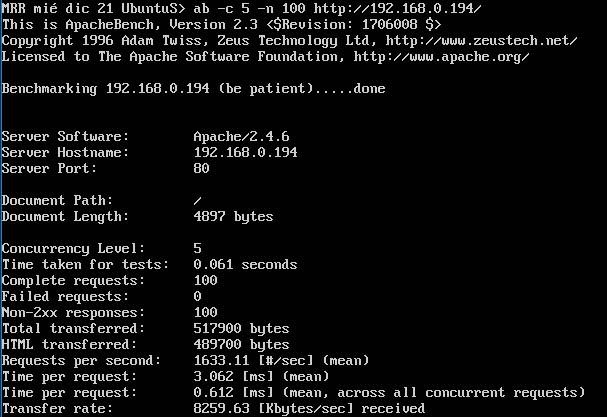
\includegraphics[scale=0.9]{figuras/ejercicio2/figura2-1.png} 
	\caption{Prueba de ab contra una máquina} 
	\label{fig:figura2-1}
\end{figure}

\newpage

\subsection{Monitorice la ejecución de ab contra alguna
	máquina (cualquiera) ¿cuántas “tareas” crea ab en el cliente?}

En este estudio el cliente va a ser la máquina de Ubuntu Server cuya IP se muestra en la Figura \ref{fig:figura2-3} y el servidor va a ser la máquina de CentOS.

\begin{figure}[H] %con el [H] le obligamos a situar aquí la figura
	\centering
	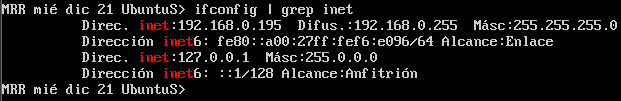
\includegraphics[scale=0.9]{figuras/ejercicio2/figura2-3.png} 
	\caption{IP de la máquina de Ubuntu Server} 
	\label{fig:figura2-3}
\end{figure}
\vspace{-10pt}
Para esta prueba se ha abierto una consola en el cliente con el gestor de procesos \textbf{top} \cite{enlace5} especificándole el nombre de usuario dueño del proceso que se busca, en este caso \textbf{www-data}. El número total de peticiones se ha puesto bastante elevado para que dé tiempo de sobra a comprobar los procesos en el cliente. La orden ha sido la siguiente:

\begin{lstlisting}[style=fich]
$ ab -c 5 -n 1000000 http://192.168.0.195/
\end{lstlisting}
\vspace{-17pt}
La ejecución de la orden anterior se muestra en la Figura \ref{fig:figura2-4}.
\begin{figure}[H] %con el [H] le obligamos a situar aquí la figura
	\centering
	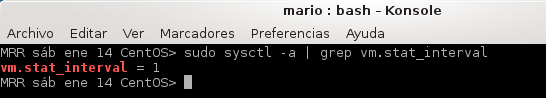
\includegraphics[scale=0.9]{figuras/ejercicio2/figura2-4.png} 
	\caption{Ejecución de \textbf{ab} en la máquina servidor} 
	\label{fig:figura2-4}
\end{figure}
\vspace{-10pt}
Viendo cómo aparecen de forma instantanea los nuevos procesos en el gestor del cliente, se puede afirmar que \textbf{ab} crea \textbf{once tareas} como puede demostrarse en la Figura \ref{fig:figura2-2}.
\begin{figure}[H] %con el [H] le obligamos a situar aquí la figura
	\centering
	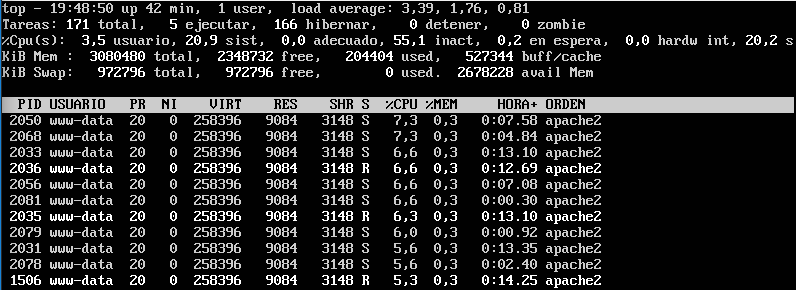
\includegraphics[scale=0.7]{figuras/ejercicio2/figura2-2.png} 
	\caption{Tareas creadas por \textbf{ab} en la máquina cliente} 
	\label{fig:figura2-2}
\end{figure}
\newpage

%----------------------------------------------------------------------------------------
%	Cuestión 3
%----------------------------------------------------------------------------------------

\section{Cuestión 3}
\subsection{Ejecute ab contra a las tres máquinas virtuales (desde el SO
	anfitrión a las máquina virtuales de la red local) una a una (arrancadas por
	separado)}

Como anfitrión se ha utilizado Windows 10 de sistema operativo y la IP es la que se muestra en la Figura \ref{fig:anfitrion}.
\begin{figure}[H] %con el [H] le obligamos a situar aquí la figura
	\centering
	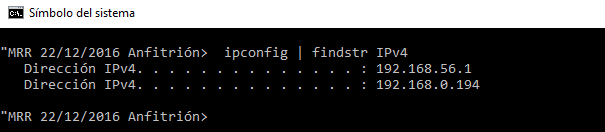
\includegraphics[scale=0.7]{figuras/ejercicio3/anfitrion.png} 
	\caption{Tareas creadas por \textbf{ab} en la máquina cliente} 
	\label{fig:anfitrion}
\end{figure}

Para la ejecución de ab en cada máquina se ha mandado la misma orden por consola, la que aparece a continuación:
\begin{lstlisting}[style=fich]
$ ab -g datos.csv -c 5 -n 10000 http://direcciónIP/ >> salida.txt
\end{lstlisting}
\vspace{-22pt}

\begin{itemize}
	\item \textbf{-g}: Este parámetro indica que se produzca un volcado de los datos en un fichero especificado para su posterior representación.
	\item \textbf{-n}: Es el número total de peticiones que se van a realizar, que en este caso siempre será \textbf{10000} para que salgan datos útiles con los que poder comparar.
	\item \textbf{-c}: Indica el número de peticiones que se ejecutarán de forma concurrente que en este caso será \textbf{5}.
	\item \textbf{http://direcciónIP/}: Donde \textbf{direccionIP} será la correspondiente a la máquina donde se va a realizar el test.
	\item \textbf{$ >> $ salida.txt}: Hace que se guarden todos los resultados finales de la ejecución en un fichero de texto.
\end{itemize}

\subsubsection{Anfitrión $ \rightarrow $ Ubuntu Server }
La dirección IP de la máquina es \textbf{192.168.0.195} como muestra la Figura \ref{fig:figura3-1-1}.

\begin{figure}[H] %con el [H] le obligamos a situar aquí la figura
	\centering
	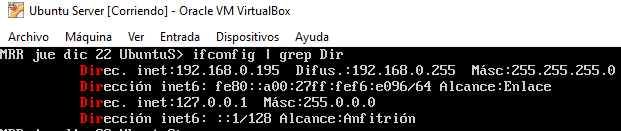
\includegraphics[scale=0.9]{figuras/ejercicio3/anf-ubuntu/figura3-1-1.png} 
	\caption{Dirección IP de la máquina Ubuntu Server} 
	\label{fig:figura3-1-1}
\end{figure}

La orden que se mencionó anteriormente queda adaptada para esta máquina como aparece en la Figura \ref{fig:figura3-1-2}.

\begin{figure}[H] %con el [H] le obligamos a situar aquí la figura
	\centering
	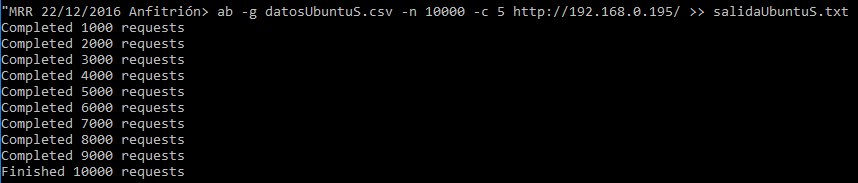
\includegraphics[scale=0.7]{figuras/ejercicio3/anf-ubuntu/figura3-1-2.png} 
	\caption{Ejecución de ab sobre la máquina Ubuntu Server} 
	\label{fig:figura3-1-2}
\end{figure}

\subsubsection{Anfitrión $ \rightarrow $ Windows Server }
La dirección IP de la máquina es \textbf{192.168.0.196} como muestra la Figura \ref{fig:figura3-2-1}.

\begin{figure}[H] %con el [H] le obligamos a situar aquí la figura
	\centering
	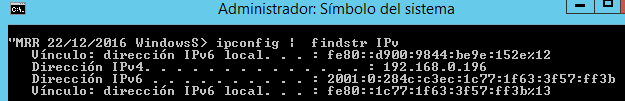
\includegraphics[scale=0.9]{figuras/ejercicio3/anf-winserver/figura3-2-1.png} 
	\caption{Dirección IP de la máquina Windows Server} 
	\label{fig:figura3-2-1}
\end{figure}

La orden que se mencionó anteriormente queda adaptada para esta máquina como aparece en la Figura \ref{fig:figura3-2-2}.

\begin{figure}[H] %con el [H] le obligamos a situar aquí la figura
	\centering
	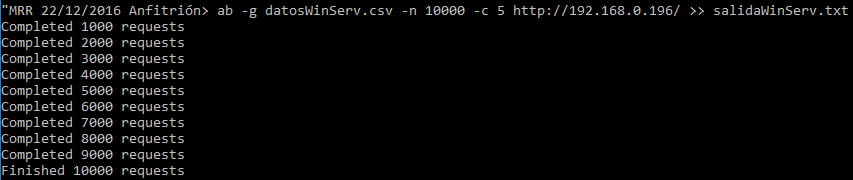
\includegraphics[scale=0.7]{figuras/ejercicio3/anf-winserver/figura3-2-2.png} 
	\caption{Ejecución de ab sobre la máquina Windows Server} 
	\label{fig:figura3-2-2}
\end{figure}

\subsubsection{Anfitrión $ \rightarrow $ CentOS }
La dirección IP de la máquina es \textbf{192.168.0.197} como muestra la Figura \ref{fig:figura3-3-1}.

\begin{figure}[H] %con el [H] le obligamos a situar aquí la figura
	\centering
	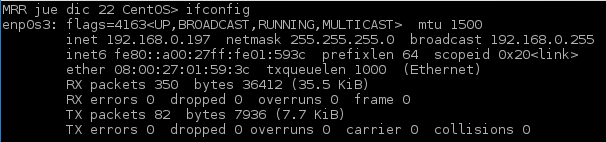
\includegraphics[scale=0.9]{figuras/ejercicio3/anf-centos/figura3-3-1.png} 
	\caption{Dirección IP de la máquina CentOS} 
	\label{fig:figura3-3-1}
\end{figure}

La orden que se mencionó anteriormente queda adaptada para esta máquina como aparece en la Figura \ref{fig:figura3-3-2}.

\begin{figure}[H] %con el [H] le obligamos a situar aquí la figura
	\centering
	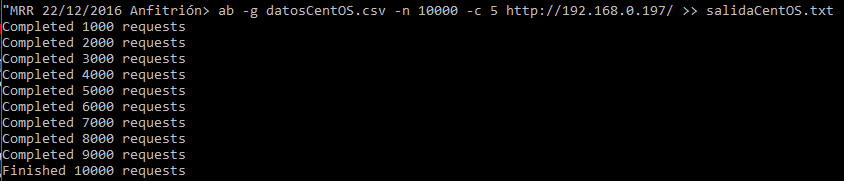
\includegraphics[scale=0.7]{figuras/ejercicio3/anf-centos/figura3-3-2.png} 
	\caption{Ejecución de ab sobre la máquina CenOS} 
	\label{fig:figura3-3-2}
\end{figure}

\newpage

\subsection{¿Cuál es la que proporciona mejores resultados? Muestre y
	coméntelos.}

Una vez obtenidos los tres ficheros de texto con los resultados se han plasmado en una tabla para poder estudiar mejor la comparativa. El resultado de ésta puede verse en la Tabla \ref{tab:addlabel}.

% Table generated by Excel2LaTeX from sheet 'Hoja1'
\begin{table}[H]
	\centering
	\begin{tabular}{lrrr}
		\textbf{Máquina} & \multicolumn{1}{l}{\textbf{CentOS}} & \multicolumn{1}{l}{\textbf{Windows Server}} & \multicolumn{1}{l}{\textbf{Ubuntu Server}} \\
		\hline
		\textbf{Server Software} & \multicolumn{1}{l}{Apache/2.4.6} & \multicolumn{1}{l}{Microsoft-IIS/8.5} & \multicolumn{1}{l}{Apache/2.4.18} \\
		\textbf{Server Hostname} & \multicolumn{1}{l}{192.168.0.197} & \multicolumn{1}{l}{192.168.0.196} & \multicolumn{1}{l}{192.168.0.195} \\
		\textbf{Server Port} & 80    & 80    & 80 \\
		\textbf{Document Path} & \multicolumn{1}{l}{/} & \multicolumn{1}{l}{/} & \multicolumn{1}{l}{/} \\
		\textbf{Document Length} (bytes) & 4897  & 701   & 11321 \\
		\textbf{Concurrency Level} & 5     & 5     & 5 \\
		\textbf{Time taken for tests (seconds)} & 9,791 & 7,647 & 10,667 \\
		\textbf{Complete requests} & 10000 & 10000 & 10000 \\
		\textbf{Failed requests} & 0     & 0     & 0 \\
		\textbf{Write errors} & 0     & 0     & 0 \\
		\textbf{Total transferred} & 51790000 & 9430000 & 115950000 \\
		\textbf{HTML transferred} & 48970000 & 7010000 & 113210000 \\
		\textbf{Requests per second} & 1021,36 & 1307,63 & 937,49 \\
		\textbf{Time per request} (ms) & 4,895 & 3,824 & 5,333 \\
		\textbf{Time per request (ms)} & 0,979 & 0,765 & 1,067 \\
		\textbf{Transfer rate} & 5165,64 & 1204,06 & 10615,37 \\
	\end{tabular}%
	\caption{Resultados de las tres máquinas}
	\label{tab:addlabel}%
\end{table}%

En la tabla puede verse cómo los resultados son totalmente distintos en los tres casos.

Para Ubuntu Server se ha obtenido tiempo el tiempo más alto de prueba (10,667s) mientras que para Windows Server el más bajo (7,647s).
\\

Con respecto a los tiempos medios por solicitud ocurre exactamente lo mismo que en el aspecto anterior, tanto en las solicitudes concurrentes como a las no concurrentes.\\

Es también muy significativa la cifra tan elevada que se ha obtenido del \textbf{total transferido} por parte de Ubuntu Server con respecto a las demás máquinas.\\

La razón por la que los resultados se hayan obtenido con de la manera anteriormente explicada se debe a que la longitud de documentos de Ubuntu Server son casi tres veces más grandes con respecto a la de CentOS y dieciséis veces más grande que la de Windows Server. Es por ello que todas las medidas de tiempo saliesen más elevadas.

% Table generated by Excel2LaTeX from sheet 'Hoja1'
\begin{table}[H]
	\centering
	\begin{tabular}{rrrr}
		\multicolumn{1}{l}{\textbf{Máquina}} & \multicolumn{1}{l}{\textbf{CentOS}} & \multicolumn{1}{l}{\textbf{Windows Server}} & \multicolumn{1}{l}{\textbf{Ubuntu Server}} \\
		\hline
		\textbf{50\%}  & 4     & 3     & 4 \\
		\textbf{66\%}  & 4     & 3     & 5 \\
		\textbf{75\%}  & 5     & 3     & 5 \\
		\textbf{80\%}  & 5     & 3     & 5 \\
		\textbf{90\%}  & 6     & 4     & 6 \\
		\textbf{95\%}  & 8     & 5     & 7 \\
		\textbf{98\%}  & 11    & 10    & 8 \\
		\textbf{99\%}  & 15    & 15    & 10 \\
		\textbf{100\%} & 36    & 54    & 32 \\
	\end{tabular}%
	\caption{Porcentaje de solicitudes atendidas dentro de un tiempo determinado (ms)}
	\label{tab:addlabel1}%
\end{table}%

Una forma más de poder visualizar los resultados es la que aparece en la Figura \ref{fig:res}. En ella pueden verse los resultados de las peticiones frente a los tiempo de respuesta medidas en microsegundos.

\begin{figure}[H] %con el [H] le obligamos a situar aquí la figura
	\centering
	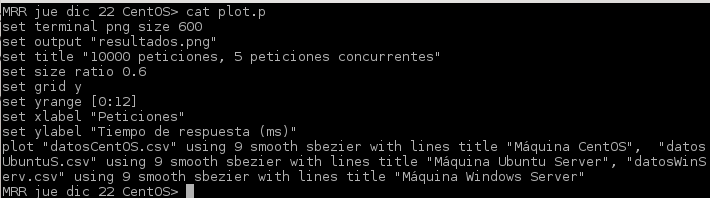
\includegraphics[scale=0.8]{figuras/ejercicio3/archivoPlot.png} 
	\caption{Archivo para la representación de los datos por gnuplot} 
	\label{fig:plot}
\end{figure}

Para esta representación se ha utilizado Gnuplot \cite{enlace6}. Ahora se utilizarán los archivos con extensión \textbf{.csv} obtenidos anteriormente en las ejecuciones que serán llamadas a través de un pequeño script de ejecución en gnuplot.
El script puede verse desglosado en la Figura \ref{fig:plot}
\\

Por tanto, la representación que ofrece la Figura \ref{fig:res} a simple vista puede distraer el resultado real obtenido en las pruebas, ya que puede parecer que la máquina CenOS es la que mayores tiempos a necesitado. No obstante, con la ayuda de la Tabla \ref{tab:addlabel} se puede afirmar que la máquina que ha obtenido mayores tiempos ha sido la de Ubuntu Server mientras que la de Windows Server ha sido la que ha requerido menos.

\begin{figure}[H] %con el [H] le obligamos a situar aquí la figura
	\centering
	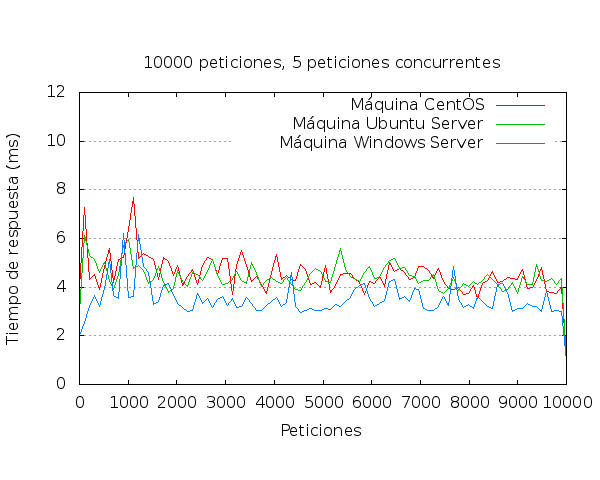
\includegraphics[scale=0.7]{calc/resultados.png} 
	\caption{Peticiones frente a tiempos de respuesta} 
	\label{fig:res}
\end{figure}

%----------------------------------------------------------------------------------------
%	Cuestión 3
%----------------------------------------------------------------------------------------

\section{Cuestión 4}
\subsection{Instale y siga el tutorial en
	\url{http://jmeter.apache.org/usermanual/build-web-test-plan.html}
	realizando capturas de pantalla y comentándolas. En vez de usar la web de
	jmeter, haga el experimento usando sus máquinas virtuales ¿coincide con
	los resultados de ab?}

Para que al final se puedan comparar los datos con los obtenidos anteriormente con ab, se ha realizado el tutorial sobre el mismo sistema operativo (Windows 10). Para ello ha bastado con descargar \textbf{JMeter} desde su página oficial \cite{enlace7} y abrir el binario \textbf{jmeter.bat} después de descomprimir el paquete.
\\

Una vez en la ventana principal, se siguen los pasos que se proporcionan en el tutorial de la página \cite{enlace8}
\begin{figure}[H] %con el [H] le obligamos a situar aquí la figura
	\centering
	\includegraphics[scale=0.5]{figuras/ejercicio4/figura1.png} 
	\caption{Ventana principal de JMeter} 
	\label{fig:figura4-1}
\end{figure}

En primer lugar se añade un nuevo grupo de hilos. Para ello se accede a través de \textbf{Editar} $ \rightarrow $ \textbf{Añadir} $ \rightarrow $ \textbf{Hilos} $ \rightarrow $ \textbf{Grupos de Hilos}, tal y como se ve en la Figura \ref{fig:figura4-2}.

\begin{figure}[H] %con el [H] le obligamos a situar aquí la figura
	\centering
	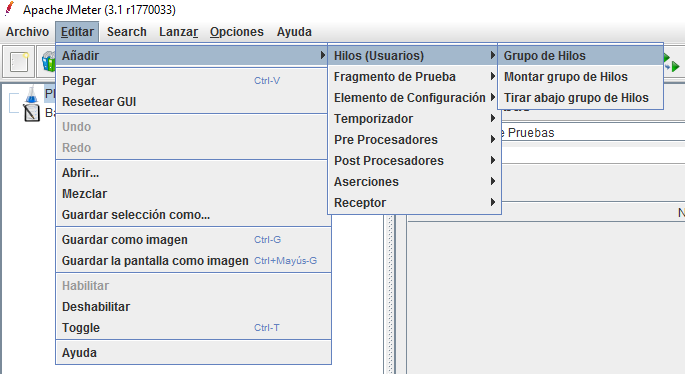
\includegraphics[scale=0.8]{figuras/ejercicio4/figura4-2.png} 
	\caption{Añadir grupo de hilos en JMeter} 
	\label{fig:figura4-2}
\end{figure}

Una vez el Grupo de Hilos añadido hay que espeficirle (Figura \ref{fig:figura4-3}) el número de éstos, que será de cinco como antes, y el contador del bucle que será dos como indica el tutorial.

\begin{figure}[H] %con el [H] le obligamos a situar aquí la figura
	\centering
	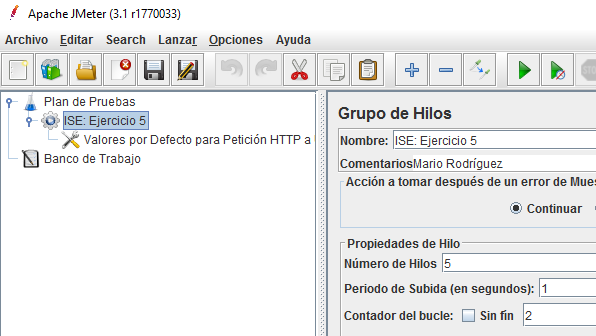
\includegraphics[scale=0.8]{figuras/ejercicio4/figura4-3.png} 
	\caption{Añadir grupo de hilos en JMeter} 
	\label{fig:figura4-3}
\end{figure}

A continuación se añaden los valores por defecto para petición HTTP. Esto se consigue mediante \textbf{Editar} $ \rightarrow $ \textbf{Añadir} $ \rightarrow $ \textbf{Elemento de Configuración} $ \rightarrow $ \textbf{Valores por defecto para Petición HTTP}, tal y como se ve en la Figura \ref{fig:figura4-4}.

\begin{figure}[H] %con el [H] le obligamos a situar aquí la figura
	\centering
	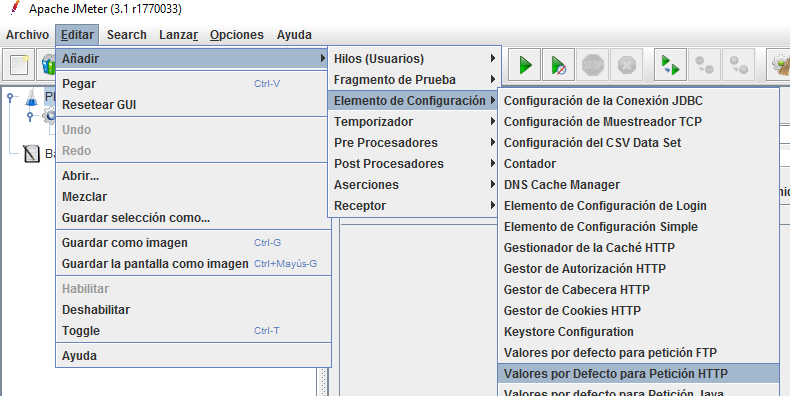
\includegraphics[scale=0.7]{figuras/ejercicio4/figura4-4.png} 
	\caption{Valores por defecto para petición HTTP en JMeter} 
	\label{fig:figura4-4}
\end{figure}

En esta ocasión solo hay que especificarle la dirección a la que se va a realizar la prueba, que ahora será \textbf{192.168.0.195} la correspondiente a la máquina Ubuntu Server y como puede verse en la Figura \ref{fig:figura4-5}.

\begin{figure}[H] %con el [H] le obligamos a situar aquí la figura
	\centering
	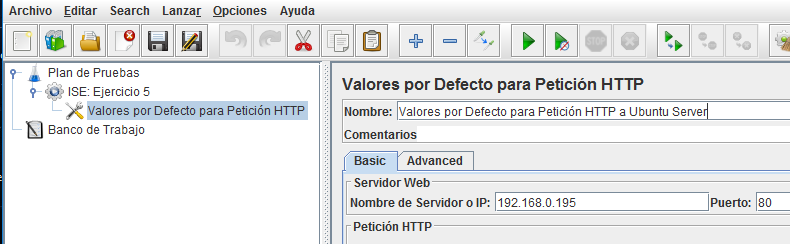
\includegraphics[scale=0.7]{figuras/ejercicio4/figura4-5.png} 
	\caption{Valores por defecto para petición HTTP en JMeter} 
	\label{fig:figura4-5}
\end{figure}

Ahora se añadirá un gestor de cookies HTTP, como indica el siguiente paso en el tutorial. A esto se accede a través de \textbf{Editar} $ \rightarrow $ \textbf{Añadir} $ \rightarrow $ \textbf{Elemento de Configuración} $ \rightarrow $ \textbf{Gestor de Cookies HTTP}, tal y como se ve en la Figura \ref{fig:figura4-6} .

\begin{figure}[H] %con el [H] le obligamos a situar aquí la figura
	\centering
	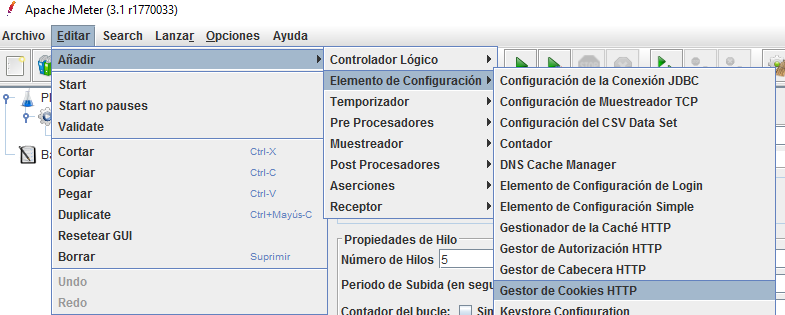
\includegraphics[scale=0.7]{figuras/ejercicio4/figura4-6.png} 
	\caption{Gestor de Cookies HTTP en JMeter} 
	\label{fig:figura4-6}
\end{figure}

El siguiente paso es añadirle la configuración de petición HTTP. A ésta se llega mediante 
\textbf{Editar} $ \rightarrow $ \textbf{Añadir} $ \rightarrow $ \textbf{Muestreador} $ \rightarrow $ \textbf{Petición HTTP}, tal y como se ve en la Figura \ref{fig:figura4-7}.

\begin{figure}[H] %con el [H] le obligamos a situar aquí la figura
	\centering
	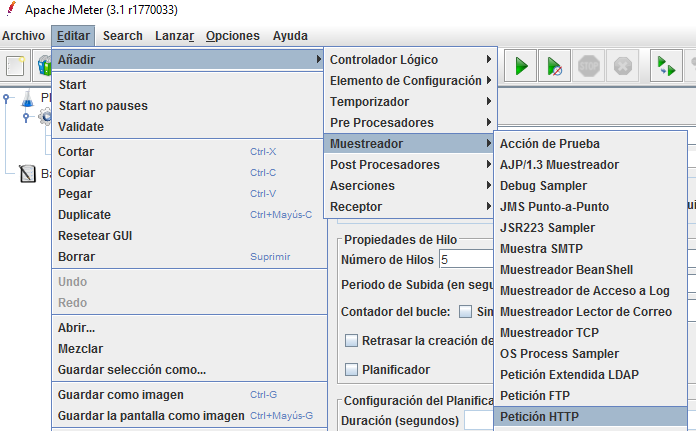
\includegraphics[scale=0.8]{figuras/ejercicio4/figura4-7.png} 
	\caption{Petición HTTP en JMeter} 
	\label{fig:figura4-7}
\end{figure}

Aquí sólo hay que indicarle la ruta de acceso que en este caso será \textbf{/index.html} como se muestra en la Figura \ref{fig:figura4-8}.

\begin{figure}[H] %con el [H] le obligamos a situar aquí la figura
	\centering
	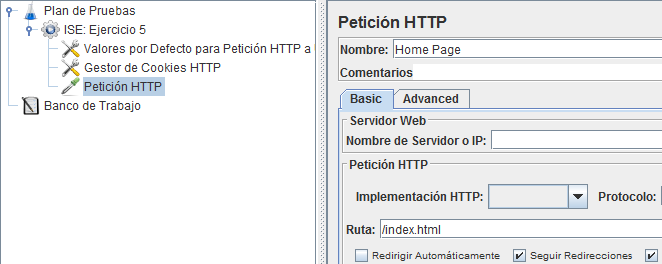
\includegraphics[scale=0.8]{figuras/ejercicio4/figura4-8.png} 
	\caption{Petición HTTP en JMeter} 
	\label{fig:figura4-8}
\end{figure}

Por último, solo falta elegir el método en el que se van a representar los resultados de las pruebas. En el tutorial indica que se haga mediante \textbf{Gráfico de resultados}, que se encuentra en \textbf{Editar} $ \rightarrow $ \textbf{Añadir} $ \rightarrow $ \textbf{Receptor} $ \rightarrow $ \textbf{Gráfico de resultados}, tal y como se ve en la Figura \ref{fig:figura4-7}

\begin{figure}[H] %con el [H] le obligamos a situar aquí la figura
	\centering
	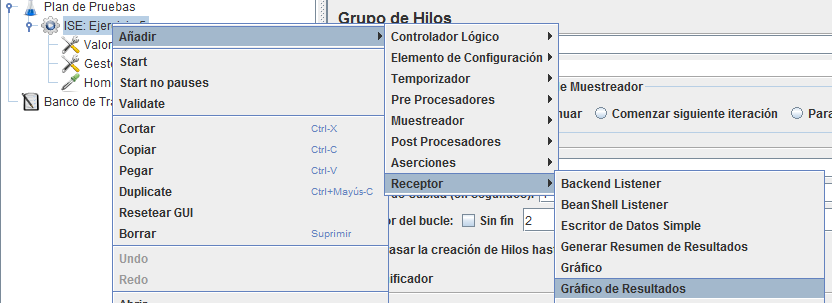
\includegraphics[scale=0.7]{figuras/ejercicio4/figura4-9.png} 
	\caption{Gráfico de resultados en JMeter} 
	\label{fig:figura4-9}
\end{figure}

Seguidos todos los pasos, ya se puede arrancar la prueba. Esto se consigue pulsando el botón \textbf{Arrancar} de color verde que se encuentra en la barra de herramientas frontal. \\

Un ejemplo de resultados en la ejecución son los que se muestran en el gráfico de la Figura \ref{fig:figura4-10}.

\begin{figure}[H] %con el [H] le obligamos a situar aquí la figura
	\centering
	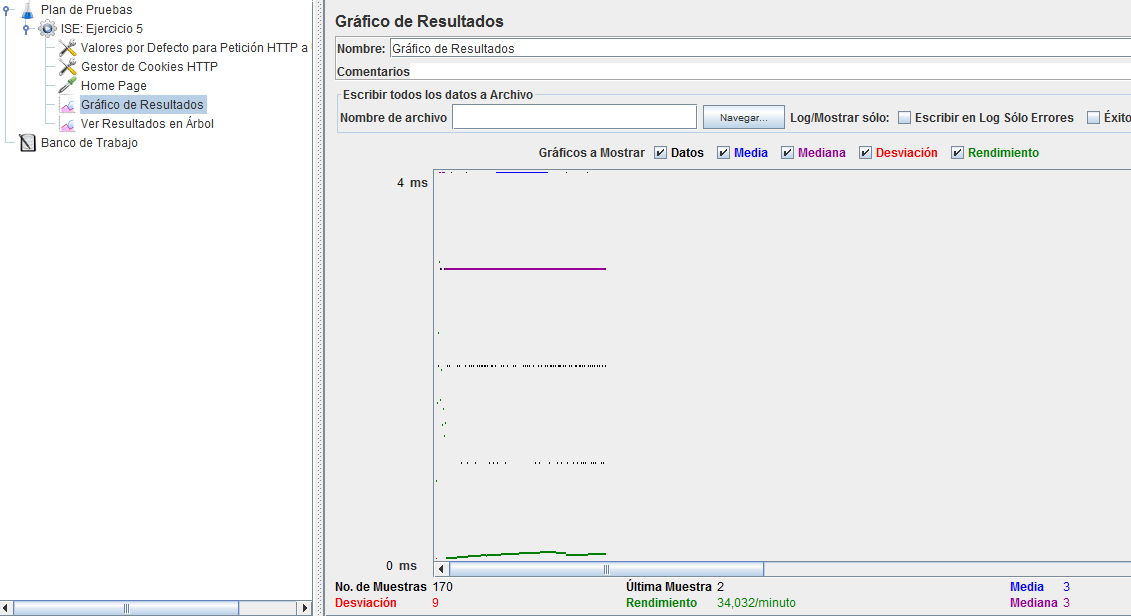
\includegraphics[scale=0.5]{figuras/ejercicio4/figura4-10.png} 
	\caption{Gráfico de resultados en JMeter} 
	\label{fig:figura4-10}
\end{figure}

Para poder comparar estos resultados con los obtenidos anteriormente con \textbf{ab}, ha sido necesario un método adicional para ello. Éste ha sido el de la representación de los resultados en árbol, en el que se muestran los resultados mejor clasificados en forma de tabla con visualización directa de resultados numérica. Esta representación se encuentra en la Figura \ref{fig:figura4-11}.

\begin{figure}[H] %con el [H] le obligamos a situar aquí la figura
	\centering
	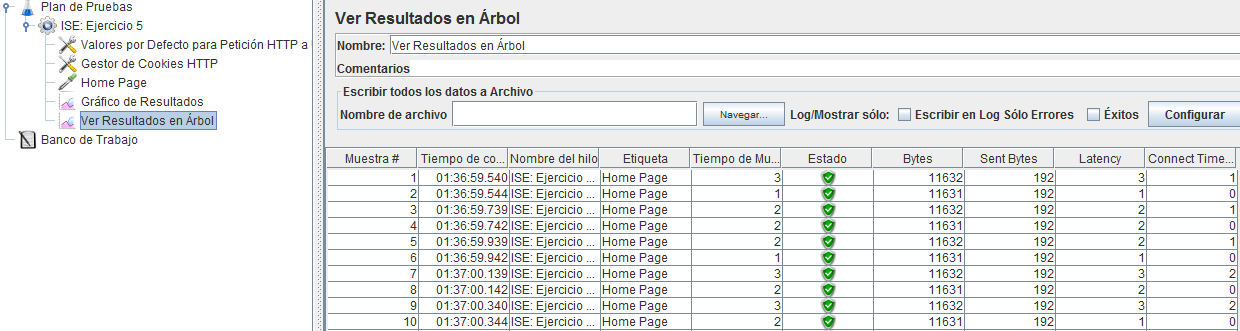
\includegraphics[scale=0.5]{figuras/ejercicio4/figura4-11.png} 
	\caption{Gráfico de resultados en árbol en JMeter} 
	\label{fig:figura4-11}
\end{figure}

Aquí si es posible ver cómo el número de bytes que se transmiten (11632) es bastante similar al que utilizaba \textbf{ab} (11321) como se mostraba en la Tabla \ref{tab:addlabel}.
\\

Con respecto a las latencias, en este caso los valores se encuentran entre 1 y 3, por lo que su media en ningún caso va a acercarse a la obtenida con \textbf{ab}, que fue sobre 5ms.
\\

Por lo que, para concluir y como respuesta a la pregunta de este guión hay que decir los resultados son cercanos a los obtenidos anteriormente con \textbf{ab} porque ya se intuía que no iban a coincidir de forma exacta al ser tratarse de pruebas distintas.

%----------------------------------------------------------------------------------------
%	Cuestión 5
%----------------------------------------------------------------------------------------

\section{Cuestión 5}
\subsection{Programe un benchmark usando el lenguaje que desee}

\subsubsection{Objetivo del benchmark}
El objetivo de este benchmark es obtener una comparación sobre el tiempo que se tarda en realizar una inserción de 10000 elementos en una tabla de \textbf{mysql} y en \textbf{mongo}.

\subsubsection{Métricas (unidades, variables, puntuaciones, etc.).}
El benchmark devuelve el tiempo transcurrido en la unidad mili-segundos, en 6 ejecuciones distintas.

\subsubsection{Instrucciones para su uso}

El requisito indispensable para poder realizar la prueba es tener tanto MySQL como Mongo instalados en el sistema. Si no es así, se debe proceder a la instalación con la ayuda del guión dos realizado en prácticas de ISE.
\\

Una vez con ambas herramientas en funcionamiento basta con ejecutar el script que se proporciona a continuación:

\lstinputlisting[style=fich]{fuentes/benchmark.sh}

El script lo que hace es la insertar los diezmil elementos seis veces en cada herramienta. Para insertar éstos se han creado dos ficheros independientes, uno para cada utilidad. 
\\

El fichero~\ref{lst:mysql} es donde se encuentra la inserción de los elementos para mysql. Su funcionamiento es el siguiente: en primer lugar comprueba que no exista una base de datos con el mismo nombre, si existiera la borra. A continuación crea la tabla e inserta todos los elementos nombrándolos \textbf{ISE} seguidos del número correspondiente a su iteración. 

\lstinputlisting[style=fich, label={lst:mysql}, caption={mysql.sql}]{fuentes/mysql.sql}

Por otro lado, el fichero~\ref{lst:mongo} hace exactamente igual que el anterior pero en la base de datos de Mongo.

\lstinputlisting[style=fich, label={lst:mongo}, caption={mysql.sql}]{fuentes/mongo.mg}

\subsubsection{Ejemplo de uso}

En una consola, dentro del directorio donde se encuentren los dos ficheros junto con el script, se ejecuta la siguiente orden:
\begin{lstlisting}[style=fich]
$ ./benchmark.sh
\end{lstlisting}
\vspace{-22pt}

Cuando termine su ejecución debe aparecer algo parecido al contenido de la Figura \ref{fig:figura5-1}. 
\begin{figure}[H] %con el [H] le obligamos a situar aquí la figura
	\centering
	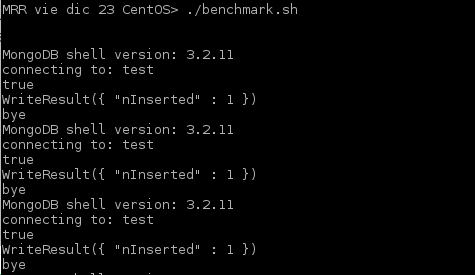
\includegraphics[scale=0.7]{figuras/ejercicio5/figura5-1.png} 
	\caption{Ejecución del script para el benchmark} 
	\label{fig:figura5-1}
\end{figure}

Ahora se comprueba que se ha creado un nuevo fichero llamado \textbf{tiempos.txt} en el directorio. En el se encuentra el volcado de los tiempos de las seis ejecuciones por herramienta. El contenido de éste debe ser similar al de la Figura \ref{fig:figura5-7}.

\begin{figure}[H] %con el [H] le obligamos a situar aquí la figura
	\centering
	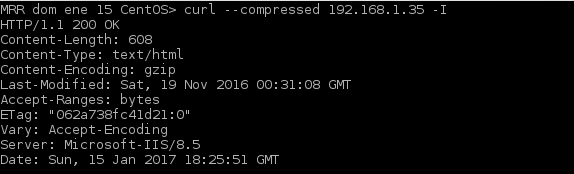
\includegraphics[scale=0.7]{figuras/ejercicio5/figura5-7.png} 
	\caption{Visualización de los tiempos del benchmark} 
	\label{fig:figura5-7}
\end{figure}

Viendo que se ha realizado una medición no nula de las pruebas, es importante comprobar que los elementos se han insertado correctamente. Para ello, en primer lugar se accede a \textbf{MySQL} mediante la orden:
\begin{lstlisting}[style=fich]
$ mysql -uroot -pPASSWORD
\end{lstlisting}
\vspace{-22pt}

Una vez dentro se visualizan las bases de datos existentes con el comando:
\begin{lstlisting}[style=fich]
$ show databases;
\end{lstlisting}
\vspace{-22pt}

En la Figura \ref{fig:figura5-2} se ve cómo se encuentra creada la nueva base de datos nombrada como \textbf{ejercicio5}.
\begin{figure}[H] %con el [H] le obligamos a situar aquí la figura
	\centering
	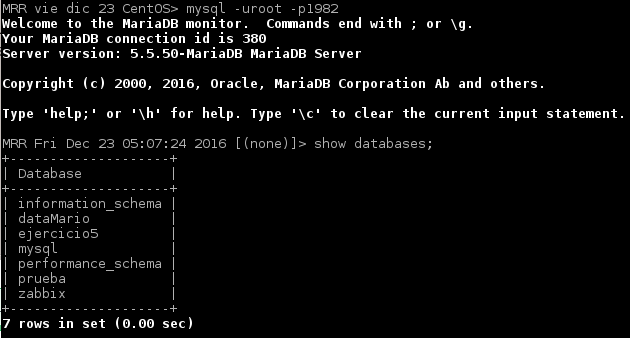
\includegraphics[scale=0.9]{figuras/ejercicio5/figura5-2.png} 
	\caption{Visualización de la nueva database en MySQL} 
	\label{fig:figura5-2}
\end{figure}

Lo siguiente es comprobar que se ha creado también la tabla dentro de la database nueva con:
\begin{lstlisting}[style=fich]
$ use ejercicio5;
$ show tables;
\end{lstlisting}
\vspace{-22pt}

En la Figura \ref{fig:figura5-3} muestra cómo se accede a la nueva database y cómo se visualizan las tablas de ésta.
\begin{figure}[H] %con el [H] le obligamos a situar aquí la figura
	\centering
	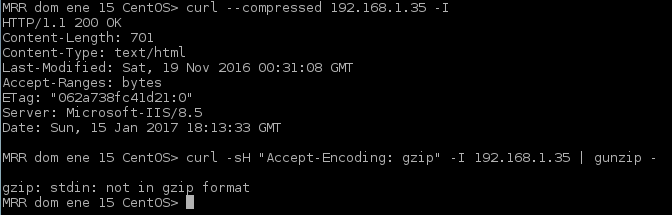
\includegraphics[scale=1]{figuras/ejercicio5/figura5-3.png} 
	\caption{Visualización de la nueva tabla en MySQL} 
	\label{fig:figura5-3}
\end{figure}

Por último, solo falta por ver que se han insertado todos y cada uno de los elementos. Ésto se consigue a través de la siguiente orden:
\begin{lstlisting}[style=fich]
$ select * from UnaTabla;
\end{lstlisting}
\vspace{-22pt}

La Figura \ref{fig:figura5-4} contiene el resultado de mostrar todos los elementos de la tabla con su número total al final.
\begin{figure}[H] %con el [H] le obligamos a situar aquí la figura
	\centering
	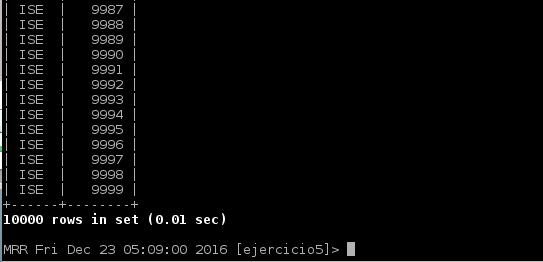
\includegraphics[scale=1]{figuras/ejercicio5/figura5-4.png} 
	\caption{Visualización de todos los elementos en MySQL} 
	\label{fig:figura5-4}
\end{figure}


De la misma forma, ahora hay que comprobar el correcto desarrollo de la prueba en \textbf{Mongo}.
\\

En primer lugar se accede a mongo a través de la consola mediante la siguiente orden:
\begin{lstlisting}[style=fich]
$ mongo
\end{lstlisting}
\vspace{-22pt}

Una vez dentro, se visualizan las colecciones y se accede a la nueva creada (\textbf{ejercicio5}), tal y como muestra la Figura \ref{fig:figura5-5}.
\begin{figure}[H] %con el [H] le obligamos a situar aquí la figura
	\centering
	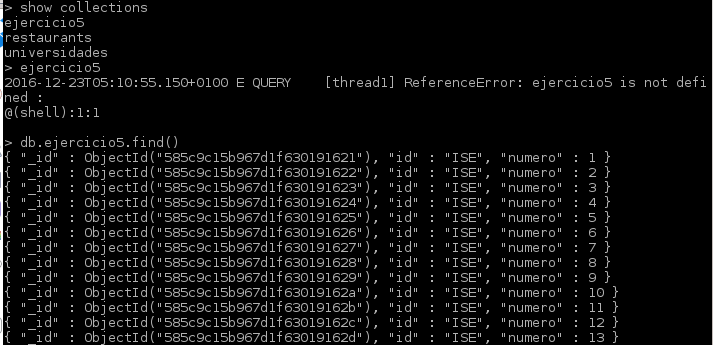
\includegraphics[scale=0.65]{figuras/ejercicio5/figura5-5.png} 
	\caption{Visualización de las colecciones en Mongo} 
	\label{fig:figura5-5}
\end{figure}

Por último, se visualizan los elementos que se han insertado a través del comando:
\begin{lstlisting}[style=fich]
$ db.ejercicio5.find()
\end{lstlisting}
\vspace{-22pt}

Como se ve en la Figura \ref{fig:figura5-6}, el número de elementos insertados es 10000. Por lo que todo se ha realizado de manera correcta.
Este último comando ha sido:
\begin{lstlisting}[style=fich]
$ db.ejercicio5.count()
\end{lstlisting}
\vspace{-22pt}

\begin{figure}[H] %con el [H] le obligamos a situar aquí la figura
	\centering
	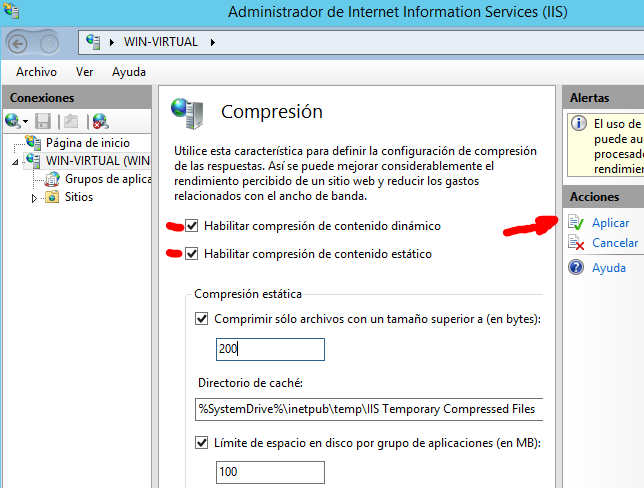
\includegraphics[scale=0.8]{figuras/ejercicio5/figura5-6.png} 
	\caption{Visualización de los elementos en Mongo} 
	\label{fig:figura5-6}
\end{figure}

\newpage

\subsubsection{Análisis de resultados}

Se quiere determinar un intervalo de confianza para el tiempo medio de este benchmark. Para ello, se han realizado varias medidas experimentales y se presentan en la Tabla \ref{tab:tiempos}.

% Table generated by Excel2LaTeX from sheet 'tiempos'
\begin{table}[H]
	\centering
	\begin{tabular}{lrr}
		\textbf{Tiempos (ms)} & \multicolumn{1}{l}{\textbf{MySQL}} & \multicolumn{1}{l}{\textbf{Mongo}} \\
		\hline
		\multicolumn{1}{r}{1} & 20270 & 5664 \\
		\multicolumn{1}{r}{2} & 25327 & 5511 \\
		\multicolumn{1}{r}{3} & 29537 & 5555 \\
		\multicolumn{1}{r}{4} & 31616 & 5359 \\
		\multicolumn{1}{r}{5} & 44045 & 5415 \\
		\multicolumn{1}{r}{6} & 41190 & 5387 \\
		\hline
		\textbf{Media} & 31997,5 & 5481,83333 \\
		\textbf{Desv\_estándar} & 9141,92257 & 116,56486 \\
		\textbf{Tamaño} & 6     & 6 \\
		\textbf{Alfa} & 0,05  & 0,05 \\
		\textbf{Intervalo de Confianza} & 7314,92714 & 93,2695998 \\
	\end{tabular}%
	\caption{Tiempos de ejecución del benchmark}
	\label{tab:tiempos}%
\end{table}%

Repasando los apuntes de clase, se ha podido llegar a cada una de estas conclusiones, tomando las fórmulas y las explicaciones necesarias.\\

Por tanto, hay un 95\% de probabilidad de que el tiempo medio real se encuentre en los intervalos:

\begin{center}
	MySQL: $ 31997,5 \pm \dfrac{7314,92714}{\sqrt{6}}t \frac{0.05}{2},6-1 = [32090,8044]ms$

Mongo: $ 5481,83333 \pm \dfrac{93,2695998}{\sqrt{6}}t \frac{0.05}{2},6-1 = [5483,02302]ms$
\end{center}
Se distribuye según la distribución \textbf{t-Student} con n-1 grados de libertad. 

Siendo \textbf{d} y \textbf{s} la media y la desviación típica muestrales, respectivamente.\\

Viendo los resultados se puede afirmar que Mongo es casi 6 veces más rápido que MySQL para esta prueba en concreto.

\newpage

%----------------------------------------------------------------------------------------
%	Referencias
%----------------------------------------------------------------------------------------
%------------------------------------------------

\bibliography{citas} %archivo citas.bib que contiene las entradas 
\bibliographystyle{plain} % hay varias formas de citar

\end{document}
